\section{Evaluation}

  The present section aims at evaluating on a COTS platform the benefits brought by SchIM (w.r.t. memory isolation) and to demonstrate the good behaviour of the different embedded policies. Therefore, we have integrated the SchIM IP on the PL side of a Xilinx ZCU102 development board, featuring a Xilinx Zynq UlraScale+ XCZU9EG SoC. For this work, we evaluate SchIM using synthetic benchmarks, real benchmarks issued from the San Diego Vision Benchmark Suite (SD-VBS) \cite{SD-VBS} and combinations of the two.
  
  The present section is organised as follows. Firstly, in subsection \ref{subsection:considered-architecture}, the exact SchIM configuration on the ZCU102 development board is discussed. Thereafter, a full assessment of the board capabilities with and without SchIM is provided in subsection \ref{subsec:platform-capabilities-and-performance-degradation}. In subsection \ref{subsec:internal-behaviour-of-schim}, an analysis of the SchIM module behaviour is presented. Finally, a demonstration of the memory isolation enabled by SchIM using real benchmark applications is provided.

  \subsection{Considered architecture}
    \label{subsection:considered-architecture}

  \subsection{Platform Capabilities and performance degradation}
    \label{subsec:platform-capabilities-and-performance-degradation}
    Intuitively and as discussed in \cite{PLIM20}, redirecting the traffic coming from the cores cluster to the PL side has a cost. In fact, the PL side running at a lower frequency and being further away on the System-on-Chip, one core will experience both a bigger latency and a smaller throughput. On the other hand, by redirecting the traffic to the PL side, we can achieve higher system predictability.
    
    In order to weight up the pro and the cons of these two orthogonal objectives, we have computed the throughput of one \emph{core under analysis}, here core 0 (noted $C_{0}$), for different configurations. The result of this experiment is display in Figure \ref{fig:bandwidth_comparison}. The configurations are a combination of a varying amount of cores competing (x axis) and different path between the cores cluster to the main memory (the different bars). More accurately, we consider five paths (i) all the cores target the main memory (referred to as \emph{Normal Route}), (ii) all the cores target a single HPM port, like they would in PLIM \cite{PLIM20} (referred to as \emph{PL Loop-back}), (iii) all the cores target the \schim IP configured to apply FP (referred to as \emph{SchIM FP}), (iv) all the cores target the \schim IP configured to apply TDMA (referred to as \emph{TDMA}) and (v) all the cores target the \schim IP configured to apply TS (referred to as \emph{SchIM MG}). These configurations are compared with respect to the throughput (expressed in MBps) that the core under analysis (i.e., core 0) experiences (y axis).
    
    From the Figure \ref{fig:bandwidth_comparison}, one can observe that in general, the throughput experienced by the core under analysis (i.e., $C_{0}$) is high and that, regardless of the contention level, the bandwidth remains high. As mentioned earlier, redirecting the cores traffic through the PL side has a cost. In fact, in the case with no contention (the left most bar cluster), the bandwidth experienced by $C_{0}$ when redirecting the traffic to a simple loop-back, is four times smaller than the normal route.
    Using the left most bar cluster, one can also observe the overhead introduced by having \schim on the memory loop-back. The overhead is approximatly of ?? MBps.
    While the throughput in the case of a \emph{PL loop-back} is bigger, it also falls as soon as the contention level increases.
    On the other hand, the \schim IP manages to preserve the same bandwidth, with only small interferences being observed in the most challenging scenario (the right most bar cluster). In other words, \schim guarantees isolation of the cores w.r.t. the bus usage.
     
    \begin{figure}
      \centering
      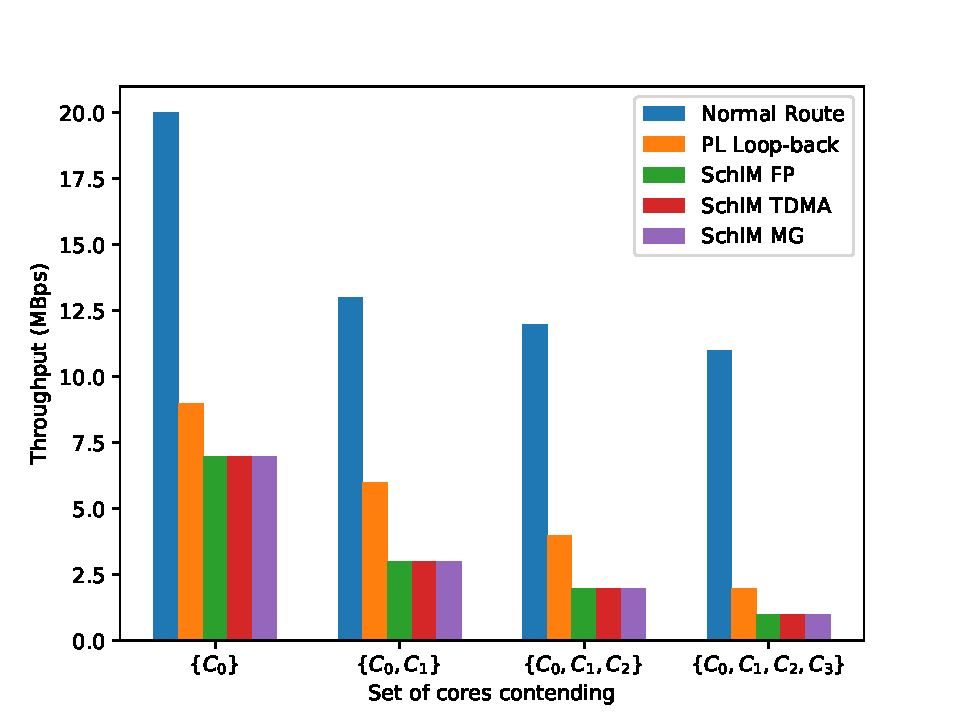
\includegraphics[scale=0.5]{images/bw_comparisons.pdf}
      \caption{Board bandwidth}
      \label{fig:bandwidth_comparison}
    \end{figure}

  \subsection{Internal Behaviour of SchIM}
    \label{subsec:internal-behaviour-of-schim}
    Here, show and emphasize on the behaviour of SchIM with Fig.\ref{fig:schim_behaviour}
    \begin{enumerate}
      \item Description of the figures
        \begin{itemize}
          \item objective
          \item technical details on how
          \item Subfigure 1
          \item Subfigure 2
          \item Subfigure 3
        \end{itemize}
      \item FP
        \begin{itemize}
          \item 
        \end{itemize}
      \item TDMA
        \begin{itemize}
          \item 
        \end{itemize}
      \item MG
        \begin{itemize}
          \item 
        \end{itemize}
    \end{enumerate}
    \todo[inline]{Here, we use the trace snapshots}
    \begin{figure}
      \centering
      \begin{subfigure}{0.5\textwidth}
        \centering
        % include first image
        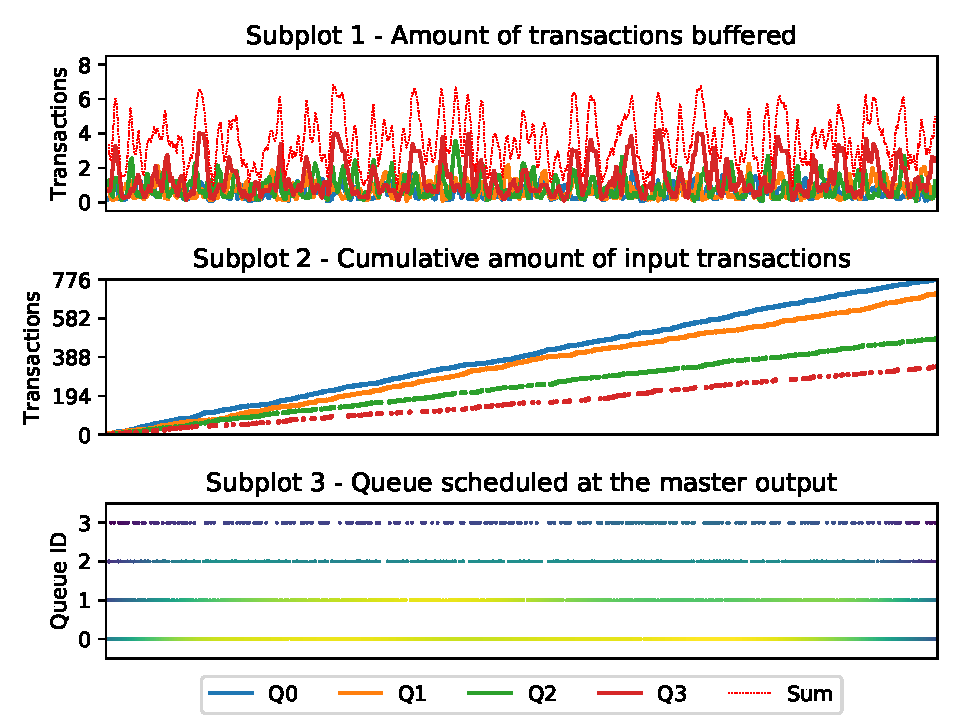
\includegraphics[scale=0.55]{images/SchIM_FP_buffering.pdf}
        \caption{FP with ordering $C_{0} \succ C_{1} \succ C_{2} \succ C_{3}$}
        \label{fig:schim_behaviour_fp}
      \end{subfigure}
      %\hfill
      \begin{subfigure}{0.5\textwidth}
        \centering
        % include second image
        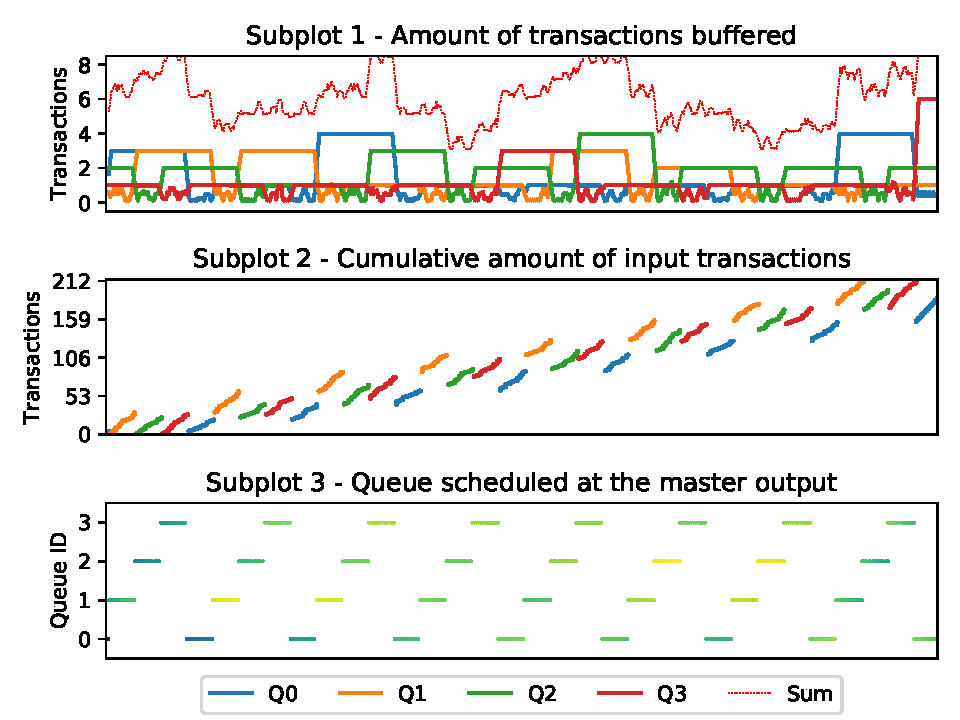
\includegraphics[scale=0.55]{images/SchIM_TDMA_buffering.pdf}
        \caption{TDMA with slots of 512 clock cycles}
        \label{fig:schim_behaviour_tdma}
      \end{subfigure}
      %\hfill
      \begin{subfigure}{0.5\textwidth}
        \centering
        % include second image
        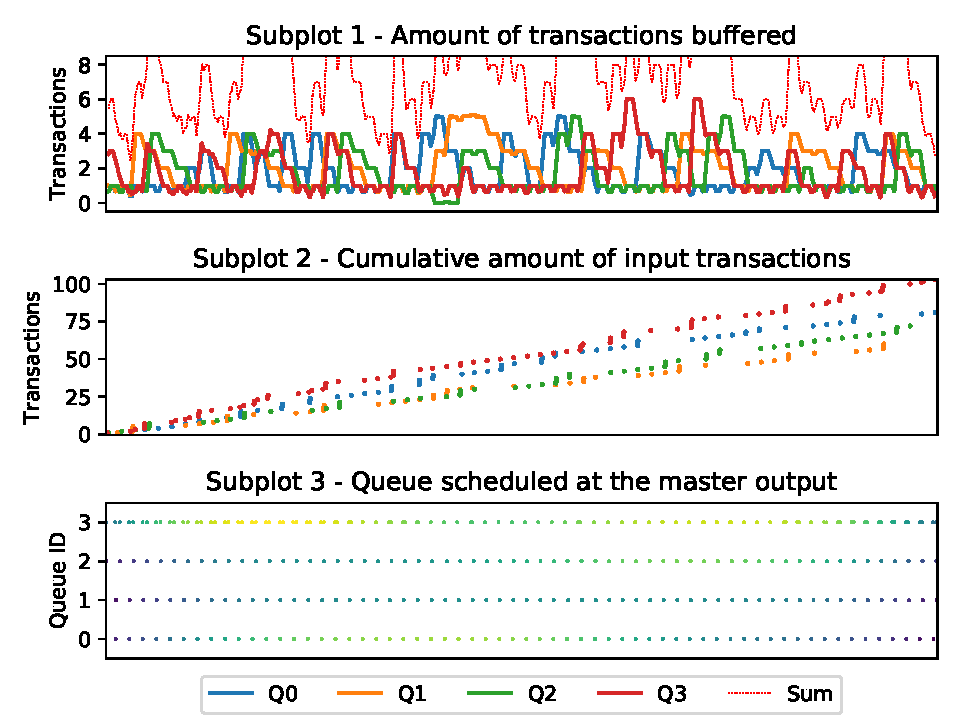
\includegraphics[scale=0.55]{images/SchIM_MG_buffering.pdf}
        \caption{MG with min. period of 256 clock cycles}
        \label{fig:schim_behaviour_mg}
      \end{subfigure}
      \caption{Trace snapshot of SchIM for the three implemented policies}
      \label{fig:schim_behaviour}
      \todo[inline]{TODO: The plots have to be reworked.}
    \end{figure}

  \subsection{Memory Isolation}
    Here, prove that SchIM enables us to isolate the cores. We need a bunch of benchmarks competing with mem-bombs on the remaining cores. We will try:
    \begin{itemize}
      \item FP:~ The benchmark running alone with the highest priority VS. the same setup with mem-bombs
      \item TDMA:~ The benchmark running alone with all the cores having a slot of the same size VS. the same setup with mem-bombs
      \item MG:~ The benchmark running alone with all the cores having a given periodicity VS. the same setup with mem-bombs
    \end{itemize}
